\documentclass{article}
\usepackage{graphicx}
\usepackage{bm}
\usepackage{amsmath}
\usepackage{amssymb}
\usepackage[toc,page]{appendix}
\usepackage{listings}
\usepackage{color}
\usepackage{listings}
\usepackage{fullpage}
\usepackage{mathtools}
\numberwithin{equation}{subsection}

\definecolor{mygreen}{rgb}{0,0.6,0}
\definecolor{mygray}{rgb}{0.5,0.5,0.5}
\definecolor{mymauve}{rgb}{0.58,0,0.82}

\lstset{ %
  backgroundcolor=\color{white},   % choose the background color; you must add \usepackage{color} or \usepackage{xcolor}
  basicstyle=\footnotesize,        % the size of the fonts that are used for the code
  breakatwhitespace=false,         % sets if automatic breaks should only happen at whitespace
  breaklines=true,                 % sets automatic line breaking
  captionpos=b,                    % sets the caption-position to bottom
  commentstyle=\color{mygreen},    % comment style
  deletekeywords={...},            % if you want to delete keywords from the given language
  escapeinside={\%*}{*)},          % if you want to add LaTeX within your code
  extendedchars=true,              % lets you use non-ASCII characters; for 8-bits encodings only, does not work with UTF-8
  frame=single,	                   % adds a frame around the code
  keepspaces=true,                 % keeps spaces in text, useful for keeping indentation of code (possibly needs columns=flexible)
  keywordstyle=\color{blue},       % keyword style
  language=Octave,                 % the language of the code
  otherkeywords={*,...},            % if you want to add more keywords to the set
  numbers=left,                    % where to put the line-numbers; possible values are (none, left, right)
  numbersep=5pt,                   % how far the line-numbers are from the code
  numberstyle=\tiny\color{mygray}, % the style that is used for the line-numbers
  rulecolor=\color{black},         % if not set, the frame-color may be changed on line-breaks within not-black text (e.g. comments (green here))
  showspaces=false,                % show spaces everywhere adding particular underscores; it overrides 'showstringspaces'
  showstringspaces=false,          % underline spaces within strings only
  showtabs=false,                  % show tabs within strings adding particular underscores
  stepnumber=2,                    % the step between two line-numbers. If it's 1, each line will be numbered
  stringstyle=\color{mymauve},     % string literal style
  tabsize=2,	                   % sets default tabsize to 2 spaces
  title=\lstname                   % show the filename of files included with \lstinputlisting; also try caption instead of title
}

\begin{document}

\title{Discrete Ordinates}
\author{Edward Norris}

\maketitle

\begin{abstract}
The abstract text goes here.
\end{abstract}

\tableofcontents

\section{CODE}
Consider that we have the following variables, $\Psi$ which is a function of $x$, $y$, $z$, $E$, and $\hat{\Omega}$. Further, we have the in-flux variables $\Psi_{x-in}$, $\Psi_{y-in}$, and $\Psi_{z-in]}$. 

Given:
\begin{itemize}
\item A list of all energies, $\{E\}$
\item A list of all directions in the quadrature, $\{\Omega\}$
\item A mapping from $r$ to zone number, $\mathcal{Z}(r)$
\item Lists of direction cosines, $\mu(\Omega)$, $\xi(\Omega)$, and $\eta(\Omega)$
\item A map of $r$ to voxel volume, $V(r)$
%\item A list of all $x$, $y$, and $z$ voxel centers, $X$, $Y$, and $Z$
\item A mapping of weights for the quadrature, $\omega(\Omega)$
\item A mapping of scatter cross sections in zone $\mathcal{Z}(r)$ from energy $E'$ to $E$, $\Sigma_s(\mathcal{Z}(r), E' \rightarrow E)$
\item A list of total cross sections in zone $\mathcal{Z}(r)$ at energy $E$, $\Sigma_T(\mathcal{Z}(r), E)$
\item The surface area of all voxels, $A_{xy}(r)$, $A_{yz}(r)$, $A_{xz}(r)$
\end{itemize}

\pagebreak
\begin{lstlisting}[escapeinside={(*}{*)}]
function sweep()

  # Knowns
  (*$V(r)$*)  # [cm^3] Volume of cell ijk
  (*$A_{xy}(\Omega,i,j), A_{yz}(\Omega,j,k), A_{xz}(\Omega,i,k)$*)  # [cm^2] Area of each face of cell ijk
  (*$S_x(E, r)$*)  # [#] External source
  # Unknowns
  (*$\phi(r, E) = \vec{0}$*)    # Scalar flux
  (*$\Psi(r, \Omega, E) = \vec{0}$*)  # Angular flux
  
  for every (*$E \in \{E\}$*) in descending order
    while not converged
      (*$\phi^{i-1}(r) = \phi^{i+1}(r)$*)
      (*$S(r) = \vec{0}$*)
      for every (*$E' >= E$*)
        for every cell (*$ijk$*)
          (*$S(ijk) = S(ijk) + 1/4\pi \phi(E', ijk)*\Sigma_s(\mathcal{Z}(ijk), E')*V(ijk)$*)
      for every cell (*$ijk$*)
        (*$S(ijk) = S(ijk) + S_{x}(ijk)$*)
      (*$\phi^{i+1} = \vec{0}$*)
      for every (*$\Omega \in Q$*) in any order
        (*$i_0 = f(\mu(\Omega))$*)
        (*$\Delta i = f(\mu(\Omega))$*)
        (*$j_0 = f(\xi(\Omega))$*)
        (*$\Delta j = f(\xi(\Omega))$*)
        (*$k_0 = f(\eta(\Omega))$*)
        (*$\Delta k = f(\eta(\Omega))$*)
        for every cell (*$ijk$*) starting at (*$(i_0, j_0, k_0)$*) in direction (*$<\Delta i, \Delta j, \Delta k>$*)
          if (*$i \in \partial$*)
            (*$\phi_{x+} = 0$*)
          else
            (*$\phi_{x+} = \phi_{x-}(i\pm 1, j, k)$*)    
          if (*$j \in \partial$*)
            (*$\phi_{y+} = 0$*)
          else
            (*$\phi_{y+} = \phi_{y-}(i, j \pm 1, k)$*) 
          if (*$k \in \partial$*)
            (*$\phi_{z+} = 0$*)
          else
            (*$\phi_{z+} = \phi_{z-}(i, j, k \pm 1)$*)     
          
          (*$n = S(ijk) + A_{yz}(\Omega, j,k)\phi_{x+} + A_{xz}(\Omega, i, k) \phi_{y+} + A_{xy}(\Omega, i,j)\phi_{z+}$*)
          (*$d = V(ijk)*\Sigma_t(\mathcal{Z}(ijk), E) + A_{yz}(\Omega, j, k) + A_{xz}(\Omega, i, k) + A_{xy}(\Omega, i, j)$*)
          (*$\Psi_0 = n/d$*)
          (*$\Psi(E, \Omega, ijk) = \Psi_0$*)
          (*$\phi_{x-}(ijk) = 2\Psi_0 - \phi_{x+}$*)
          (*$\phi_{y-}(ijk) = 2\Psi_0 - \phi_{y+}$*)
          (*$\phi_{z-}(ijk) = 2\Psi_0 - \phi_{z+}$*)
          (*$\phi^{i+1}(ijk) = \phi^{i+1} + \omega(\Omega)\Psi(e, \Omega, ijk)$*)
        for every cell (*$ijk$*)
          (*$\phi(E, ijk) = \phi^{i+1}(ijk)$*)
        EMIT (*$\phi(E, ijk)$*)
      (*$\epsilon = max((\phi^{i+1} - phi^{i-1})/\phi^{i+1})$*)
      
      for every cell (*$ijk$*)
        (*$\phi(E, ijk) = \phi^{i+1}(ijk)$*)
  output time to completion
\end{lstlisting}

\pagebreak
\begin{lstlisting}[escapeinside={(*}{*)}]
function octant1()

  for (*$x \in X$*) in ascending order
    for (*$y \in Y$*) in ascending order
      for (*$z \in Z$*) in ascending order
            
        (*$S$*) = totalScatter((*$x, y, z, \Omega, E$*))            
            
        # Get the in-flux from the previous out-flux
        (*$\Psi_{x-in}(x, y, z, E, \Omega) \leftarrow \Psi_{x-out}(x-\Delta x, y, z, E, \Omega)$*)
        (*$\Psi_{y-in}(x, y, z, E, \Omega) \leftarrow \Psi_{x-out}(x, y-\Delta y, z, E, \Omega)$*)
        (*$\Psi_{z-in}(x, y, z, E, \Omega) \leftarrow \Psi_{x-out}(x, y, z-\Delta z, E, \Omega)$*)
              
        # Calculate the angular flux
        (*$n \leftarrow S + 2\mu(\Omega)A_{yz}(y,z)\Psi_{x-in}(x,y,z,E,\Omega) + $*)
               (*$2\xi(\Omega)A_{xz}(x,z)\Psi_{y-in}(x,y,z,E,\Omega) + $*)
               (*$2\eta(\Omega)A_{xy}(x,y)\Psi_{z-in}(x,y,z,E,\Omega)$*)
        (*$d \leftarrow 2\mu(\Omega)A_{yz}(y,z) + 2\xi(\Omega)A_{xz}(x,z) + 2\eta(\Omega)A_{xy}(x,y) + \Sigma_T(\mathcal{Z}(r), E)$*)
        (*$\Psi(x, y, z, E, \Omega) \leftarrow n/d $*)
              
        # Calculate the out-flux
        (*$\Psi_{x-out}(x, y, z, E, \Omega) \leftarrow 2 \Psi(x, y, z, E, \Omega) - \Psi_{x-in}(x, y, z, E, \Omega)$*)
        (*$\Psi_{y-out}(x, y, z, E, \Omega) \leftarrow 2 \Psi(x, y, z, E, \Omega) - \Psi_{y-in}(x, y, z, E, \Omega)$*)
        (*$\Psi_{z-out}(x, y, z, E, \Omega) \leftarrow 2 \Psi(x, y, z, E, \Omega) - \Psi_{z-in}(x, y, z, E, \Omega)$*)
            
        # Increment the scalar flux
        (*$\phi(x, y, z, E) \leftarrow \phi(x, y, z, E) + \omega(\Omega) \Psi(x, y, z, E, \Omega)$*)
\end{lstlisting}

\pagebreak
\begin{lstlisting}[escapeinside={(*}{*)}]
function totalScatter((*$r, \Omega, E$*))

  # Assume a point source at (*\color{mygreen} $r_0$*) with energy (*\color{mygreen} $E_0$*) and strength (*\color{mygreen} $S_0$*) particles / sec
  (*$S_x \leftarrow 0$*)
  if (*$r = r_0$*) and (*$E = E_0$*)
    (*$S_x \leftarrow (1/4\pi) \times S_0$*)

  (*$S_D \leftarrow 0$*)
  for (*$E' \in \mathcal{E} | E' \geq E$*)
    (*$S_D = S_D + (1/4\pi) \times \phi(r, \Omega, E') \times \Sigma_s(\mathcal{Z}(r), E', E) \times V(r)$*)
    
  (*$S_T = S_x + S_D$*)
  return (*$S_T$*)
\end{lstlisting}

The indexing scheme is as follows: E, A, x, y, z, l, m

\section{Introduction}
This document will teach you everything you need to know about the Boltzmann Equation from its derivation to the details of its implementation in computer code.

\section{Mathematical Development}

\subsection{The Boltzmann Equation}

The time dependent gamma transport equation can be written as

\begin{equation} \label{eq:boltz_t_dep}
\begin{split}
	&\left[ \frac{1}{v(E)} \frac{\partial}{\partial t} + \hat{\Omega} \cdot \nabla + \Sigma_t(\boldsymbol{r}, E, t) \right]
	\psi(\boldsymbol{r}, E, \hat{\Omega}, t) = \\
	&\int_{4 \pi} \int_0^\infty \Sigma_s(\boldsymbol{r}, E' \rightarrow E, \hat{\Omega}' \rightarrow \hat{\Omega}, t) \psi(\boldsymbol{r}, E', \hat{\Omega}', t) dE' d\hat{\Omega}' + S(\boldsymbol{r}, E, \hat{\Omega}, t)
\end{split}
\end{equation}

However, we are typically not concerned with the transient case in medical diagnostic imaging. We are more interested in the steady state case. The time independent form of Eq. \ref{eq:boltz_t_dep} is written as

\begin{equation} \label{eq:boltz}
\begin{split}
	&\left[ \hat{\Omega} \cdot \nabla + \Sigma_t(\boldsymbol{r}, E) \right]
	\psi(\boldsymbol{r}, E, \hat{\Omega}) = \\
	&\int_{4 \pi} \int_0^\infty \Sigma_s(\boldsymbol{r}, E' \rightarrow E, \hat{\Omega}' \rightarrow \hat{\Omega}) \psi(\boldsymbol{r}, E', \hat{\Omega}') dE' d\hat{\Omega}' + S(\boldsymbol{r}, E, \hat{\Omega})
\end{split}
\end{equation}

The following sections show how Eq.~\ref{eq:boltz} is discretized.

\subsection{Angular Discretization}
The coordinate system used in DOCTORS is shown in Fig.~\ref{fig:coord_sys}. A discrete set of $N_a$ angles ($\Omega_{a} \quad a = 0 \ldots N_a-1$) is selected to represent continuous directional space. Particles are transported only along these discrete directions form one voxel to adjacent voxels.

The $S_N$ quadrature is implemented in DOCTORS. There are many different quadrature sets, the $S_N$ quadratures were selected because they are easy to implement, rotationally symmetric, and the most commonly used in production discrete ordinate solvers. This enables simple, direct comparison to other solvers. Arbitrary quadratures are permissible in a plain text file supplied by the user enabling other quadratures.

\begin{figure}
    \centering
    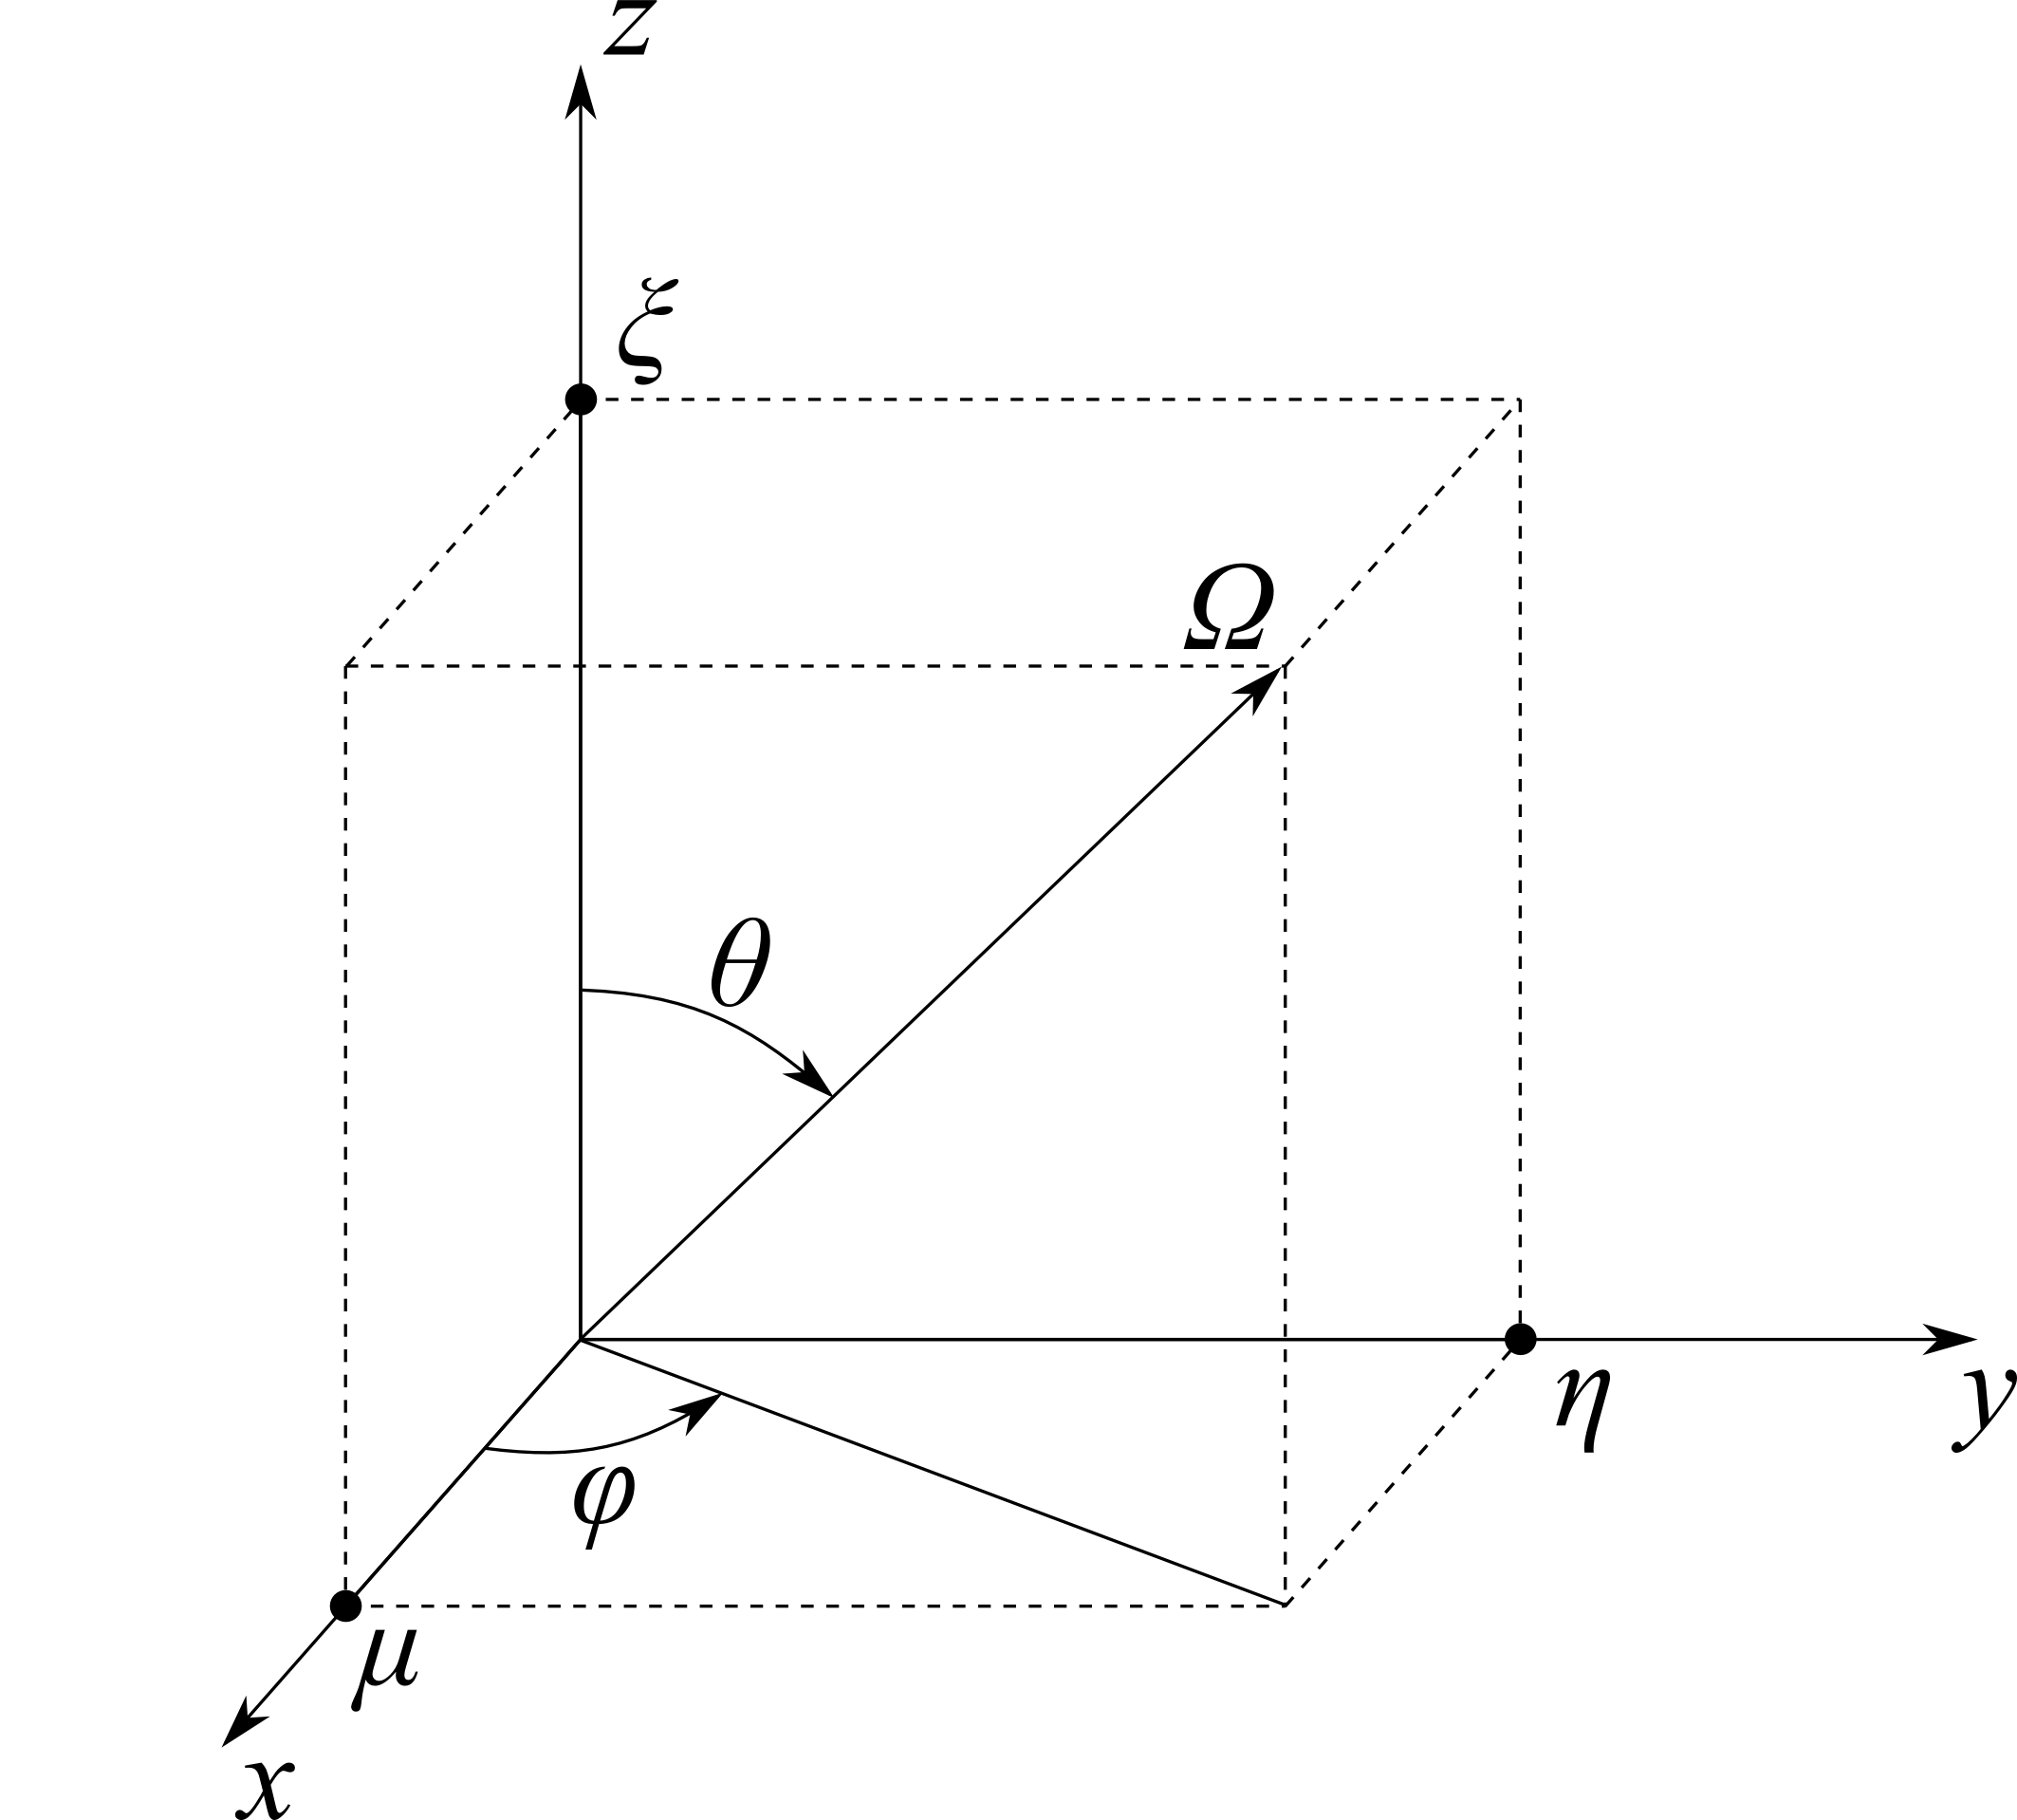
\includegraphics[width=3.0in]{figs/coord_sys}
    \caption{The coordinate system used in DOCTORS. Given an arbitrary direction, $\Omega$, $\mu$, $\eta$, and $\xi$ are its direction cosines with respect to the $x$, $y$, and $z$ axes respectively. $\varphi$ is the azimuthal angle (with respect to $x$ and the d $\theta$ is the polar angle (with respect to $z$).}
    \label{fig:coord_sys}
\end{figure}

Each discrete angle is associated a weight. The weights are designed with the angles such that once a discrete quadrature is selected, integration over continuous space becomes integration in discrete space approximated by Eq.~\ref{eq:disc_int}.

\begin{equation} \label{eq:disc_int}
\int_{4 \pi} f(\hat{\Omega}) d\Omega \approx \sum_{a=0}^{N_a-1} f(\hat{\Omega}_a) \omega_a
\end{equation}

Discretizing Eq.~\ref{eq:boltz} in angular space gives Eq.~\ref{eq:boltz_a} where the angle is denoted by subscript $a$.

\begin{equation} \label{eq:boltz_a}
\begin{split}
	&\left[ \hat{\Omega}_a \cdot \nabla + \Sigma_t(\boldsymbol{r}, E) \right]
	\psi_{a}(\boldsymbol{r}, E) = \\
	&\sum_{a=0}^{N_a-1} \int_0^\infty \Sigma_{s, a, a'}(\boldsymbol{r}, E' \rightarrow E) \psi_{a'}(\boldsymbol{r}, E') dE' \omega_a + S_a(\boldsymbol{r}, E)
\end{split}
\end{equation}

\subsection{Energy Discretization}

Continuous energy is discretized into $G$ groups indexed from 0 to $G-1$. Upscatter is assumed to be negligible. Therefore, Eq.~\ref{eq:boltz_a} becomes the energy discretized Eq.~\ref{eq:boltz_e} where the group number is indexed by superscript $g$. The group structure is shown in Fig.~\ref{fig:energy_groups}.

\begin{equation} \label{eq:boltz_e}
	\left[ \hat{\Omega}_a \cdot \nabla + \Sigma_t^g(\boldsymbol{r}) \right]
	\psi_{a}^{g}(\boldsymbol{r}) = 
	\sum_{a=0}^{N_a-1} \sum_{g'=g}^{G-1} \Sigma_{s, a, a'}^{g, g'}(\boldsymbol{r}) \psi_{a'}^{g'}(\boldsymbol{r}) \omega_a + S_a^g(\boldsymbol{r})
\end{equation}

\begin{figure}
    \centering
    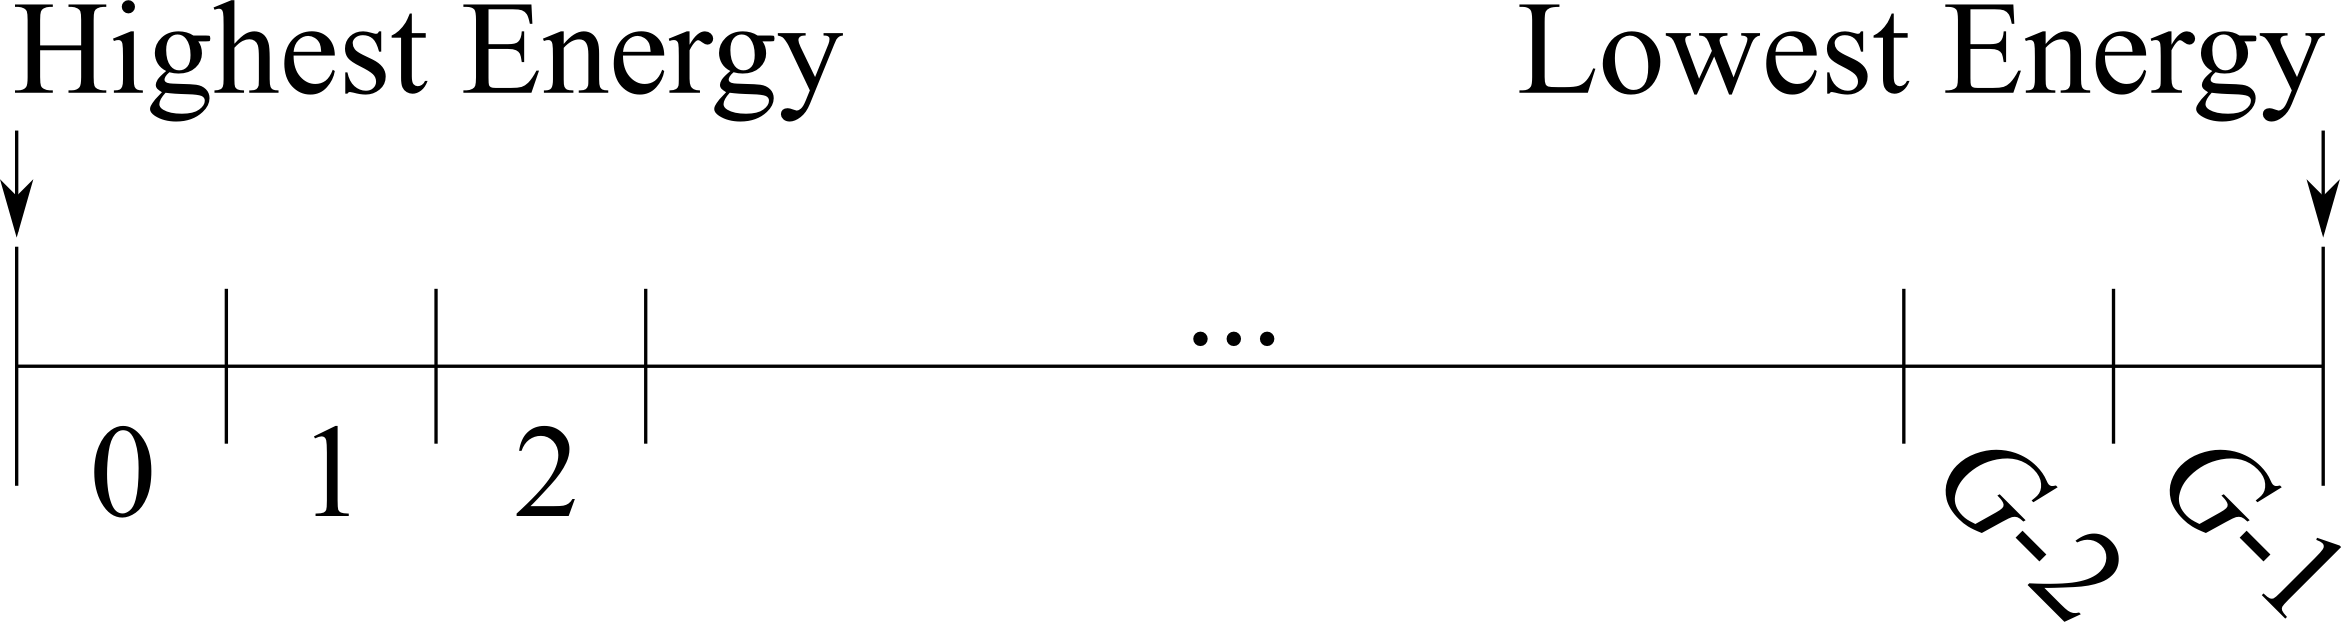
\includegraphics[width=3.0in]{figs/energy_groups}
    \caption{The energy grid structure used in DOCTORS. The highest energy group is group 0 and the lowest energy is group $G-1$.}
    \label{fig:energy_groups}
\end{figure}

\subsection{Spatial Discretization}

Finally, Eq.~\ref{eq:boltz_e} is discretized in space to give Eq.~\ref{eq:boltz_r} which is fully discretized. The problem domain is split into an evenly spaced Cartesian grid. The grid spacing between each of the spatial dimensions does not necessarily need to be uniform, but it often is in the case of CT voxel phantoms.

The problem domain must be a regular rectangular parallelpiped of size $D_x$, $D_y$, and $D_z$ in the $x$, $y$, and $z$ directions respectively. The mesh is partitioned into $N_x$, $N_y$, and $N_z$ evenly spaced bins along each direction. The total number of voxels, $N_V$ is easily computed as the multiple of each of the component directions given in Eq.~\ref{eq:n_v}.

\begin{equation} \label{eq:n_v}
	N_V = N_x N_y N_z
\end{equation}

Voxel indices are flattened according to the rule given in Eq.~\ref{eq:indx_flat}. Note that all indeces always start at zero.

\begin{equation} \label{eq:indx_flat}
	i = i_x (N_z + N_y) + i_y N_z + i_z
\end{equation}

The spatial mesh is shown in Fig.~\ref{fig:spatial_disc}. The size of each voxel in each dimension is computed by dividing the size of the problem domain along in that dimension by the number of mesh elements along the same direction. Eq.~\ref{eq:mesh_x} shows this computation for the $x$ direction. Analagous equations apply in the $y$ and $z$ directions as well.

\begin{equation} \label{eq:mesh_x}
\Delta x = \frac{D_x}{N_x}
\end{equation}

\begin{figure}
    \centering
    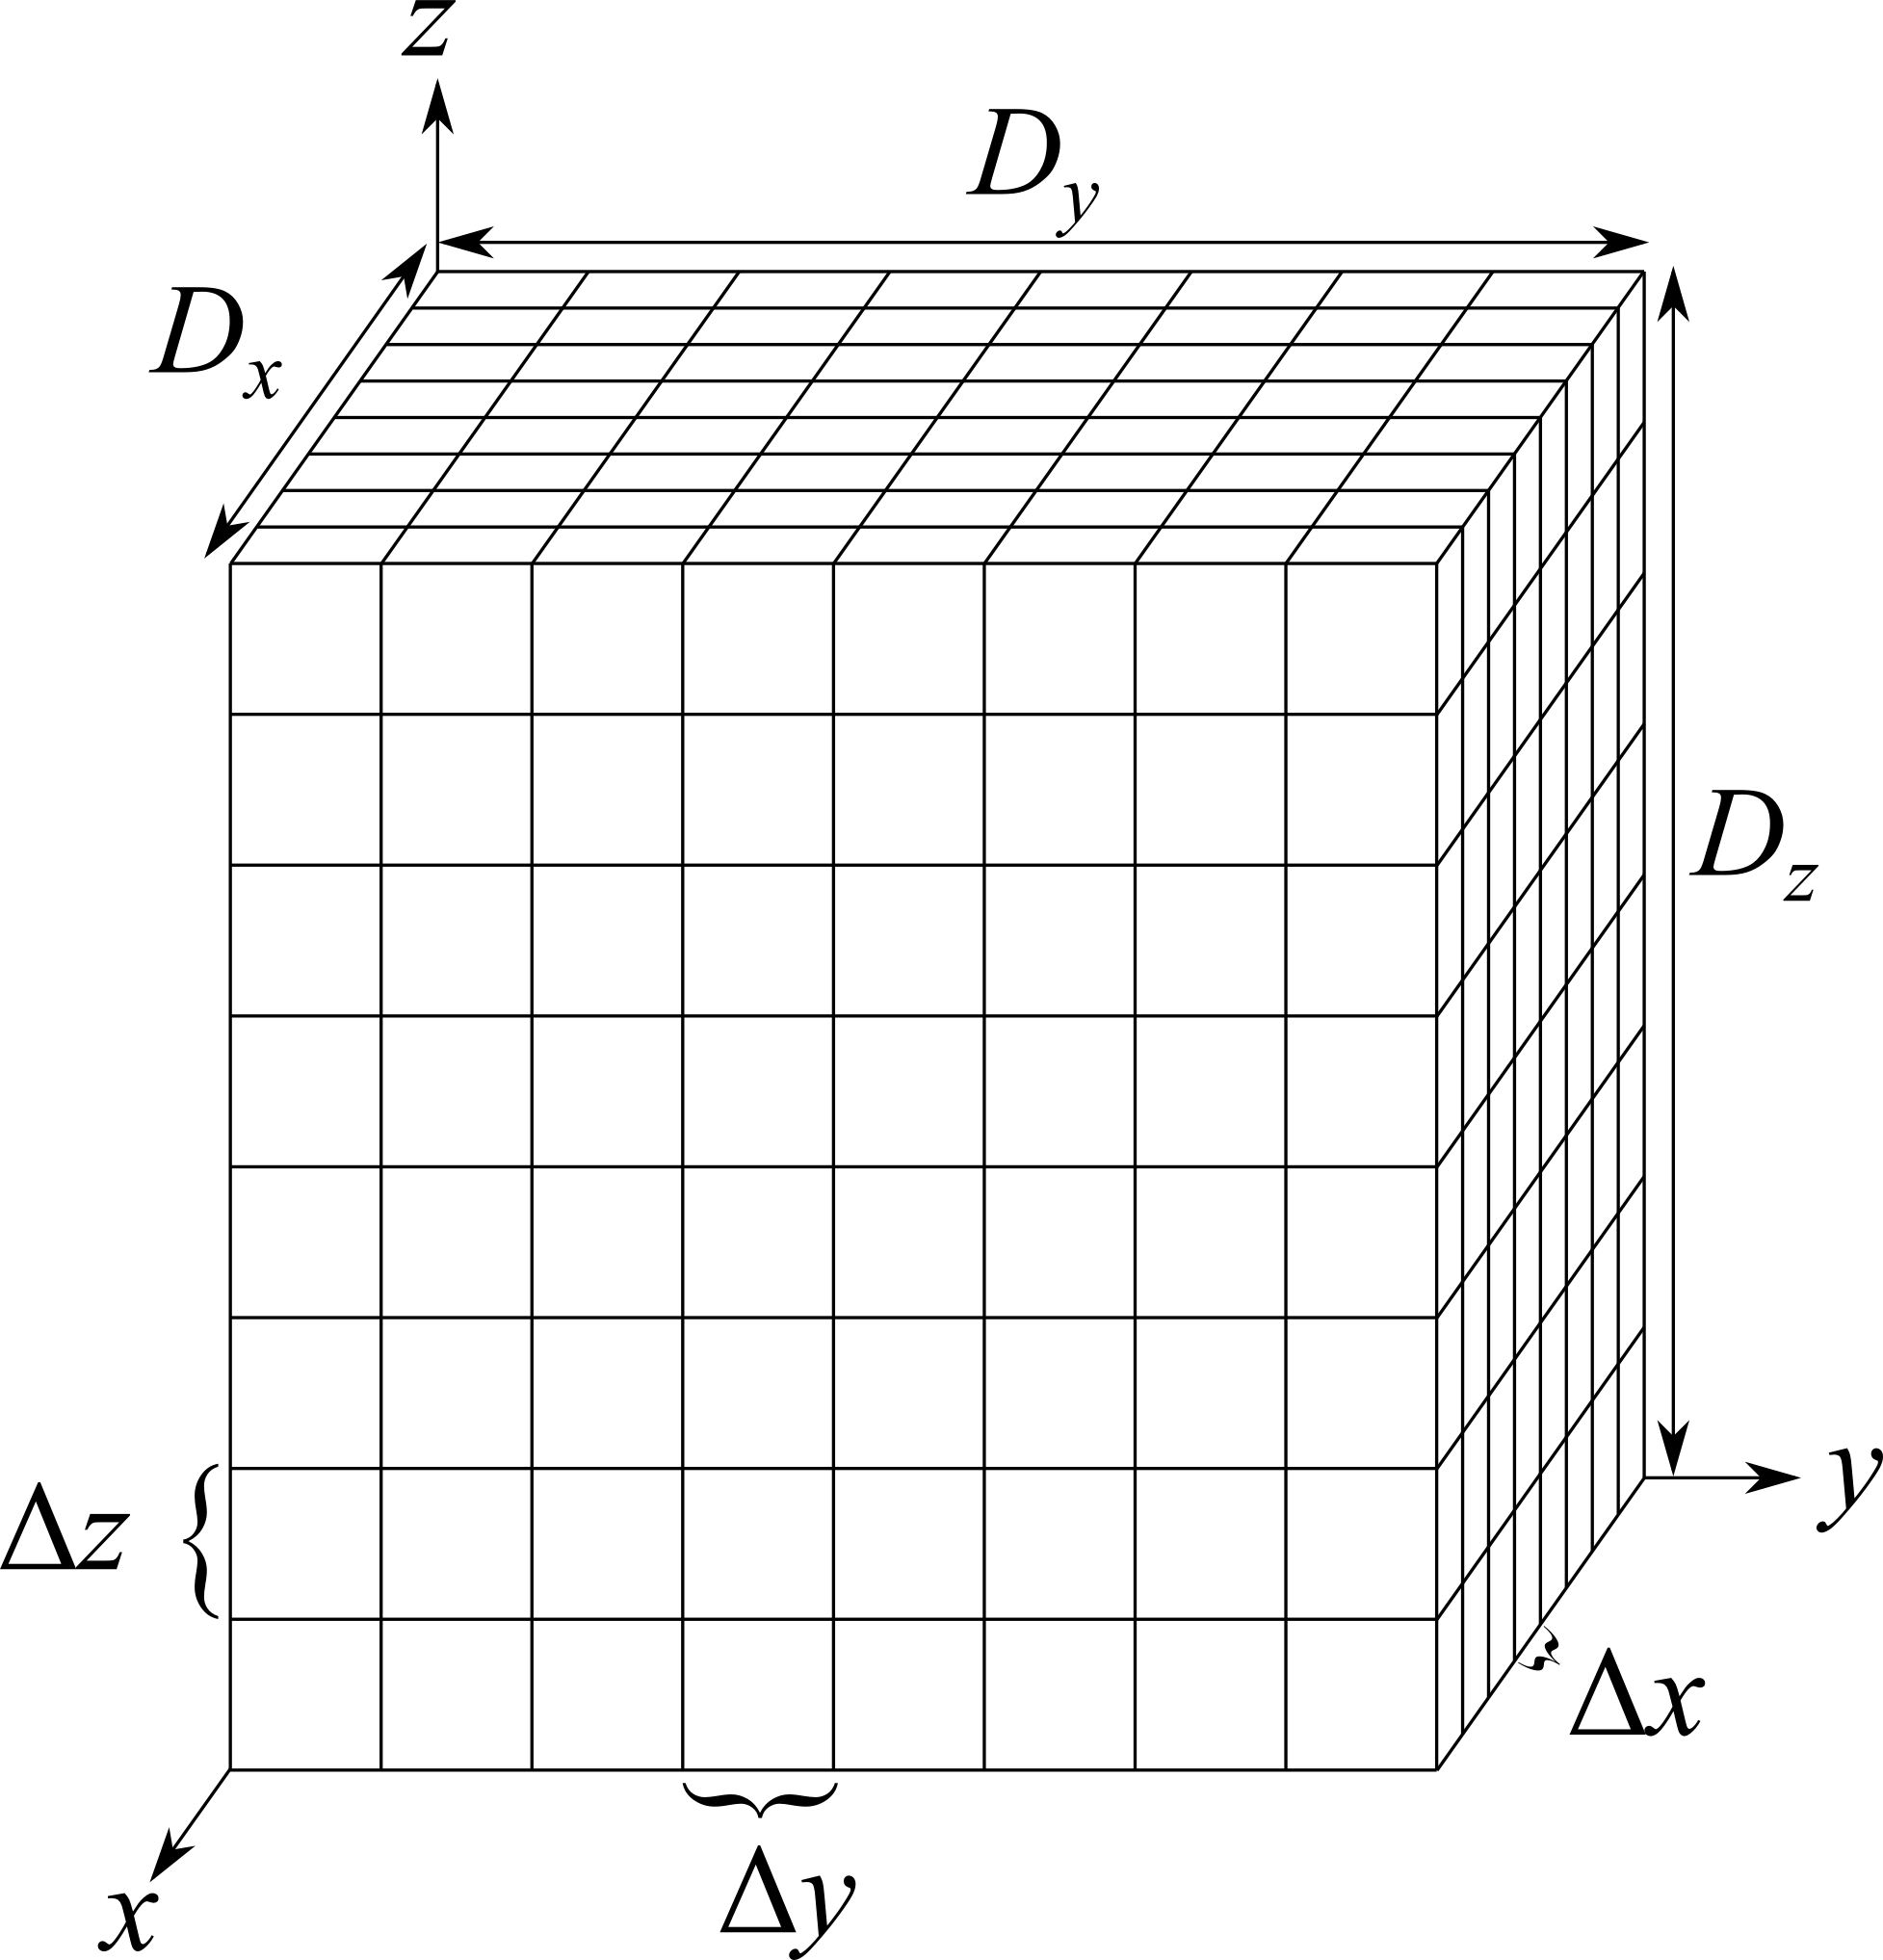
\includegraphics[width=3.0in]{figs/spatial_disc}
    \caption{The spatial mesh imposed on the problem domain.}
    \label{fig:spatial_disc}
\end{figure}


\subsection{Harmonic Approximation}
Equation \ref{eq_boltz} has a number of terms that cannot be solved directly. Instead, some numerical approximation must be used. The macroscopic scattering cross section, $\Sigma_s$ is typically expanded with a Legendre polynomial (for more information of Legendre polynomials, refer to Section \ref{sec_legendre}). The expansion is as follows:

\begin{equation} \label{eq_sigma_expansion}
\Sigma_s(\boldsymbol{r}, E' \rightarrow E, \hat{\Omega}' \rightarrow \hat{\Omega}) \approx \sum_{l=0}^L \frac{2l+1}{4 \pi} \Sigma_{s,l}(\boldsymbol{r}, E' \rightarrow E) P_l(\hat{\Omega}' \rightarrow \hat{\Omega})
\end{equation}

where $\Sigma_{s,l}$ is the expansion coefficients termed the "scattering moments." The Legendre polynomials $P_l(\hat{\Omega}' \rightarrow \hat{\Omega}$ are defined as

\begin{equation} \label{eq_harmonic}
P_l(\hat{\Omega}' \rightarrow \hat{\Omega}) = \frac{1}{2l+1}\sum_{m=-l}^l Y_{l,m}^*(\hat{\Omega}')Y_{l,m}(\hat{\Omega})
\end{equation}

The angular fluence ($\phi$) is also expanded as

\begin{equation}
\phi(\boldsymbol{r}, E', \hat{\Omega}') \approx \sum_{l=0}^L \sum_{m=-l}^l
\phi_{lm}(\boldsymbol{r}, E')Y_{lm}(\hat{\Omega}')
\end{equation}

\noindent
A source term suitable for numeric integration is then

\begin{equation}\label{eq_harmonic_simp1}
\begin{split}
\int_0^\infty dE' \int_{4 \pi} d\hat{\Omega}' \Sigma_s(\boldsymbol{r}, E' \rightarrow E, \hat{\Omega}' \rightarrow \hat{\Omega}) \phi(\boldsymbol{r}, E', \hat{\Omega}')
\approx \\
 \sum_{l=0}^L \frac{2l+1}{4 \pi} \sum_{m=-l}^l \Sigma_{s,l}^{gg'}\phi_{i,j,k,lm}^{g'}Y_{l,m}(\hat{\Omega}_n)
\end{split}
\end{equation}

Finally, substituting Eqs. \ref{eq_harmonic_simp1} and <> into <>, we arrive at

\begin{equation}\label{eq_discretized}
\begin{split}
\hat{\Omega}_n \cdot \nabla\psi_{i,j,k,n}^g + \sigma_{i,j,k}^g \psi_{i,j,k,n}^g = \\
\sum_{g' = 0}^G \sum_{l=0}^L \frac{2l+1}{4 \pi} \sum_{m=-l}^l \sigma_{s,l}^{g,g'}\psi_{i,j,k,l,m}^{g'}Y_{l,m}(\hat{\Omega}_n) + \frac{1}{4 \pi}q_{i,j,k}^g
\end{split}
\end{equation}

We can calculate the scalar flux as

\begin{equation}
\phi_{i,j,k}^g = \sum_{n=1}^{|\Omega|} w_n \psi_{i,j,k,n}^g
\end{equation}

\subsection{Discretization}
The continuous Boltzmann Equation Approximation has to be discretized in all dimensions to run on a computer.

The gradient of $\psi$ is calculated as

\begin{equation}
\nabla \psi_{i,j,k,n}^g \approx
\left\langle  
\frac{\psi_{i+1,j,k}^g - \psi_{i-1,j,k}^g}{\Delta x},
\frac{\psi_{i,j+1,k}^g - \psi_{i,j-1,k}^g}{\Delta y},
\frac{\psi_{i,j,k+1}^g - \psi_{i,j,k-1}^g}{\Delta z}
\right\rangle
\end{equation}

There are six faces on each parallelpiped with normals $<\pm 1, 0, 0>$, $<0, \pm 1, 0>$, and $<0, 0, \pm 1>$. Taking the dot product of these normals and the evaluated gradient gives

\begin{equation}
\hat{\Omega} \cdot \nabla \psi_{i,j,k}^g \approx
2 \left(
\frac{\psi_{i+1,j,k}^g - \psi_{i-1,j,k}^g}{\Delta x} +
\frac{\psi_{i,j+1,k}^g - \psi_{i,j-1,k}^g}{\Delta y} +
\frac{\psi_{i,j,k+1}^g - \psi_{i,j,k-1}^g}{\Delta z}
\right)
\end{equation}

\begin{figure}
    \centering
    \includegraphics[width=3.0in]{myfigure}
    \caption{Simulation Results}
    \label{simulationfigure}
\end{figure}

\subsection{Raytracer}
Discrete ordinate solutions greatly benefit from the presence of a raytracing algorithm to provide the uncollided flux to the solver.

The raytracer was implemented as...

When the solver is changed from isotropic to anisotropic, the raytracer must be able to not only compute the uncollided flux but compute the direction of flux in each voxel and map that onto the discrete quadrature.

To map an arbitrary direction onto a discete quadrature set, the direction is split amonst the three nearest directions in the quadrature set. Each quadrature direction is weighted. The closeness of each direction computed by calcualting the cosine of the angle between a direction $\hat{\Omega}$ and the quadrature direction $\hat{\Omega}_a$. The cosine is computed

\begin{equation}
\cos(\theta) = \hat{\Omega} \cdot \hat{\Omega}_a
\end{equation}

The three nearest points are then taken to form a triangle with the $\hat{\Omega}$ direction between them as shown in Fig. XYZ.

The area of $\triangle \mathbf{A} \mathbf{B} \mathbf{\Omega}$ is

\begin{equation}
A = |\mathbf{A}-\mathbf{B}| |\mathbf{A}-\mathbf{C}| \sqrt{1-\left[ (\mathbf{A}-\mathbf{B}) \cdot (\mathbf{A}-\mathbf{C}) \right]}
\end{equation}

Remove what is below this!

\begin{equation}
    Y_l^m(\theta, \phi)= 
\begin{cases}
\sqrt{2} K_l^m \cos(m \phi) P_l^m(\cos(\theta)),      & m > 0 \\
K_l^0 P_l^0(\cos(\theta)),              & m = 0  \\
\sqrt{2} K_l^m \sin(-m \phi) P_l^{-m}(\cos(\theta)),           & m < 0
\end{cases}
\end{equation}

where $K_l^m$ is defined as

\begin{equation}
K_l^m = \sqrt{\frac{2l+1}{4 \pi} \frac{(l-|m|)!}{(l+|m|)!}}
\end{equation}

and the associated Legendre functions are computed by the recursion

\begin{equation}
\begin{aligned}
P_0^0(x) &= 1 \\
P_m^m(x) &= (2m-1)!!(1-x^2)^{m/2} \\
P_{m+1}^m(x) &= x(2m+1)P_m^m(x) \\
P_l^m(x) &= \frac{x(2l-1)}{l-m} P_{l-1}^m (x) - \frac{l+m-1}{l-m} P_{l-2}^m (x)
\end{aligned}
\end{equation}

The spherical harmonic expansion is used to approximate a function $f$ by 

\begin{equation}
f(\theta, \phi) = \sum_{l=0}^\infty \sum_{m=-l}^l y_l^m(\theta, \phi) f_l^m
\end{equation}

which is exact when the expansion continues to infinity. However, it is trunctated at L yielding

\begin{equation}
f(\theta, \phi) \approx \sum_{l=0}^L \sum_{m=-l}^l y_l^m(\theta, \phi) f_l^m
\end{equation}

However, the value of each $f_l^m$ must be computed before the approximation can be used.

These values are computed by

\begin{equation}\label{eq:flm}
f_l^m = \int_{4 \pi} y_l^m(\theta, \phi) f(\theta, \phi) d\hat{\Omega}
\end{equation}

In the case of the raytracer solution, since \textit{only} the uncollided source is considered, the direction at any point is always precisely known, the particles are traveling away from the source point. Therefore, the function to be approximated is a Dirac delta function in the two dimensional surface of the unit sphere. Equation~\ref{eq:flm} can be reduced to

\begin{equation}
f_l^m = \int_{4 \pi} y_l^m(\theta, \phi)f(\theta_0, \phi_0) d\hat{\Omega}
\end{equation}

The property of the Dirac delta function 

\begin{equation}
\int_{-\infty}^{\infty} \delta(x_0) f(x) dx = f(x_0)
\end{equation}

can now be used which reduces Equation~\ref{eq:flm} to

\begin{equation}
f_l^m = y_l^m(\theta_0, \phi_0)
\end{equation}

The moments are related to the angular flux by

\begin{equation}
\phi_l^m(\vec{r}, E) = \int Y_l^m(\hat{\Omega} ') \psi(\vec{r}, \hat{\Omega}', E) d\hat{\Omega}'
\end{equation}

which, for the uncollided flux, becomes

\begin{equation}
\phi_l^m(\vec{r}, E) = \Psi Y_l^m(\hat{\Omega}_0)
\end{equation}

where $\Psi$ is equal to the magnitude of $\psi_{unc}$ in the $\hat{\Omega}_0$ direction.

\section{Implementation}
At this point, we have successfully developed an algorithm that can be implemented on a computer. However, there are many challenges in actually implementing this algorithm.

\subsection{Design}
Yeah, it was designed.

\subsection{Language Selection}
Yeah, it was selected.

\subsection{Salome}
We chose to use the Salome framework for numerical pre/post-processing. Salome includes a built in geometry system and meshing capabilities.

\subsection{Framework Integration}
Yeah, it was integrated

\subsection{C++ Implementation}
Yeah, it was implemented.

\begin{lstlisting}
#include <stdio.h>
#define N 10
/* Block
 * comment */

int main()
{
    int i;

    // Line comment.
    puts("Hello world!");
    
    for (i = 0; i < N; i++)
    {
        puts("LaTeX is also great for programmers!");
    }

    return 0;
}
\end{lstlisting}

\section{MPI Implementation}
MPI stands for Message Passing Interface and is the \textit{de Facto} standard for implementing parallel algorithms across multiple physical machines.

\section{GPU Implementation}
GPU stands for Graphical Processing Unit and is a collection of SIMD (single instruction multiple data) processors. Each processor operates on its own piece of data but performs the same operation each other processor in its warp is executing.

\section{Conclusion}
Hooray! It works!

\section{Appendix}

\subsection{Laplace's Equation} \label{sec_laplace}
Many physical phenomena can be described by Poisson's Equation given below.

\begin{equation} \label{eq_poisson}
\nabla^2 f = \psi
\end{equation}

Laplace's Equation is a special form of Poisson's Equation and is given by Eq. \ref{eq_laplace}.


\begin{equation} \label{eq_laplace}
\nabla^2 f = 0
\end{equation}

Laplace's equation in cartesian coordinates expands to

\begin{equation} \label{eq_laplace_cartesian}
\nabla^2 f(x, y, z) = \frac{\partial^2 f}{\partial x^2} + \frac{\partial^2 f}{\partial y^2} + \frac{\partial^2 f}{\partial z^2} = 0
\end{equation}

In cylindrical coordinates
\begin{equation} \label{eq_laplace_cylindrical}
\nabla^2 f(r, \phi, z) = \frac{1}{r} \frac{\partial}{\partial r}\left( r \frac{\partial f}{\partial r}\right) + \frac{1}{r^2}\frac{\partial^2 f}{\partial \phi^2} + \frac{\partial^2 f}{\partial z^2}
\end{equation}

In spherical coordinates
\begin{equation} \label{eq_laplace_spherical}
\nabla^2 f(\rho, \theta, \phi) = \frac{1}{\rho^2}\frac{\partial}{\partial \rho} \left( \rho^2 \frac{\partial f}{\partial \rho}\right) + \frac{1}{\rho^2 \sin \theta}\frac{\partial}{\partial \theta}\left( \sin \theta \frac{\partial f}{\partial \theta}\right) + \frac{1}{\rho^2 \sin^2 \theta} \frac{\partial^2 f}{\partial \phi^2}
\end{equation}

Any solution to Laplace's equation is known as a harmonic function. Further, if any two functions are a solution to Laplace's equation, then by the superposition principle, the summation of the two functions is also a solution to Laplace's equation.

Common solutions to Laplace's equation include

\begin{table}
\begin{center}
\label{tbl_laplace_solutions}
\caption{A list of solutions to Laplace's equation in different geometrical systems}
\begin{tabular}{|l|c|}
\hline
Cartesian & Exponential, Circular (a class of trig function), hyperbolic \\ \hline
Cylindrical & Bessel, Exponential, Circular \\ \hline
Spherical & Legendre polynomial, Power, Circular \\ \hline
\end{tabular}
\end{center}
\end{table}

\subsection{Legendre Polynomials} \label{sec_legendre}

Legendre polynomials are solutions to
\begin{equation}
P_n(x) = \frac{1}{2 \pi i} \oint \frac{1}{\sqrt{1-2\xi x + \xi^2}} \frac{1}{\xi^{n+1}} d\xi
\end{equation}



The first few such solutions are \\
$P_0(x) = 1$ \\
$P_1(x) = x$ \\
$P_2(x) = \frac{1}{2}(3x^2-1)$ \\
$P_3(x) = \frac{1}{2}(5x^3 - 3x)$ \\
$P_4(x) = \frac{1}{8}(35x^4 - 30x^2 + 3)$ \\
$P_5(x) = \frac{1}{8}(63x^5 - 70x^3 + 15x)$ \\
$P_6(x) = \frac{1}{16}(231x^6 - 315x^4 + 105x^2 - 5)$ \\

Legencre polynomials are useful for approximating functions truncated at some point. Legendre polynomials are mutually orthogonal which gives them the property

\begin{equation}
f(x) = \sum_{n=0}^\infty P_n(x)
\end{equation}

where $f(x)$ is any arbitrary function. Often, like a Fourier series which uses sin and cos instead of Legendre functions, the series is cut off at some threshold as an approximation. As an example of this, consider the function $1.75x^3 + 0.6x^2+.21x-.06$ over the domain $[2,5]$ using the first four Legendre polynomials.

The coefficients are computed

\begin{align}
k_0 &= \int_2^5 P_0(x) f(x) dx = \int_2^5  f(x) dx\\
k_1 &= \int_2^5 P_1(x) f(x) dx = \int_2^5 x f(x) dx\\
k_2 &= \int_2^5 P_2(x) f(x) dx = \int_2^5 \frac{1}{2}(3x^2-1) f(x) dx\\
k_3 &= \int_2^5 P_3(x) f(x) dx = \int_2^5 \frac{1}{2}(5x^3 - 3x) f(x) dx\\
\end{align}

These values are then used to reconstruct the original function by

\begin{equation}
f(x) \approx k_0 P_0(x) + k_1 P_1(x) + k_2 P_2(x) + k_3 P_3(x)
\end{equation}


Associated Legendre polynomials are a generalization of the Legendre polynomial and solve 

\subsection{Associated Legendre Polynomials}\label{sec:assoc_leg}

The associated Legendre polynomials are solutions to the equation 

\begin{equation}
P_l^m(x) = (-1)^m(1-x^2)^{m/2}\frac{d^m P_l(x)}{dx^m}
\end{equation}

The associated Legendre polynomials can be computed recusively by

\begin{align}
P_m^m(x) &= (-1)^m(2m-1)!!(1-x^2)^(m/2) \\
P_{m+1}^m(x) &= x(2m+1)P_m^m(x) \\
(l-m) P_l^m(x) &= x(2l-1)P_{l-1}^m(x) - (l+m-1)P_{l-2}^m(x)
\end{align}

where $x!!$ is the double factorial function defined by:

\begin{equation}
x!! = \prod_{k=0}^{\lceil x/2 \rceil - 1} x-2k
\end{equation}

For example, $5!! = 5 \times 3 \times 1 = 15$ and $6!! = 6 \times 4 \times 2 = 48$.

Some references omit the Condon-Shortley phase $(-1)^m$ while most others include it. These two are distinguished by the nomenclature

\begin{equation}
P_{lm}(x) = (-1)^m P_l^m(x)
\end{equation}

Only the more commonly found $P_l^m$ form will be used in this work.

\subsection{Spherical Harmonic Function}

Combining the associated Legendre polynomials and the sin/cos series, the spherical harmonics equations can be derived. They are orthogonal in both directions.

\begin{equation}\label{eq:spherical_harmonic}
Y_l^m(\theta, \phi) = N_l^{|m|} P_l^{|m|}(\cos \theta) e^{i m \phi}
\end{equation}

Using Euler's Equation (Eq. \ref{eq:euler}) to compute the imaginary exponent, the spherical harmonic can be expanded to Eq. \ref{eq:spherical_harmonic_exp}.

\begin{equation}\label{eq:euler}
e^{i \theta} = \cos(\theta) + i \sin(\theta)
\end{equation}

\begin{equation}\label{eq:spherical_harmonic_exp}
Y_l^m(\theta, \varphi) = N_l^{|m|} P_l^{|m|}(\cos \theta) \left[ \cos(m \phi) + i \sin(m \phi) \right]
\end{equation}

The normalization constant $N_l^m$ is defined as

\begin{equation}
N_l^m = \sqrt{(2-\delta_{m,0}) \frac{2l+1}{4 \pi} \frac{(l-m)!}{(l+m)!}}
\end{equation}

where $\delta$ is the Kronecker delta defined by

\begin{equation}
\delta_{x,y} =
\begin{cases*}
1,  \quad \text{if } x = y \\
0, \quad \text{otherwise} \\
\end{cases*}
\end{equation}

In many cases, only the real part ($y_l^m$) of the complex spherical harmonics ($Y_l^m$) are necessary. 

\begin{equation}
y_l^m =
\begin{cases*}
N_l^m P_l^m(\cos(\theta)) \cos(m\phi) & m \textgreater \, 0  \\
N_l^0 P_l^0(\cos(\theta)) & m = 0 \\
N_l^{|m|} P_l^{|m|}(\cos(\theta)) \sin(|m| \phi) & m \textless \, 0 
\end{cases*}
\end{equation}

\begin{equation}\label{eq:spherical_harmonic_xs}
\Sigma_s(\Omega \cdot \Omega') \approx \sum_{l=0}^L \sigma_l \sum_{m=-l}^l Y_l^m(\Omega)\bar{Y}_l^m(\Omega')
\end{equation}

where the over-bar denotes the complex conjugate defined by Eq.~\ref{eq:spherical_harmonic_conj}.

\begin{equation}\label{eq:spherical_harmonic_conj}
\bar{Y}_l^m(\theta, \varphi) = (-1)^{l}\sqrt{\frac{2l+1}{4 \pi}
\frac{(l-m)!}{(l+m)!}} P_l^m(\cos \theta) \left[ \cos(m \varphi) - i \sin(m \varphi) \right]
\end{equation}

Expanding the inner summation of \ref{eq:spherical_harmonic_xs} with Eq.~\ref{eq:spherical_harmonic_exp} and \ref{eq:spherical_harmonic_conj} yields:

\begin{equation}\label{eq:spherical_harmonic_xs_inner}
\begin{split}
Y_l^m(\theta, \varphi)\bar{Y}_l^m(\theta', \varphi') & = 
(-1)^{2l}\frac{2l+1}{4 \pi}
\frac{(l-m)!}{(l+m)!} P_l^m(\cos \theta) P_l^m(\cos \theta') \times \\
&\left[ \cos(m \varphi) + i \sin(m \varphi) \right] \left[ \cos(m \varphi') - i \sin(m \varphi') \right] \\
& = \frac{2l+1}{4 \pi}
\frac{(l-m)!}{(l+m)!} P_l^m(\cos \theta) P_l^m(\cos \theta') \times \\
& \left[ \cos(m \varphi) \cos(m \varphi') + i \sin(m \varphi)\cos(m \varphi') - i \sin(m \varphi') \cos(m \varphi) - i^2\sin(m \varphi) \sin(m \varphi') \right]
\end{split}
\end{equation}

The real part of the

whose real part can be expanded to

\begin{equation}
Y_l^0 = \sqrt{\frac{2l+1}{4 \pi}}P_l^0(1)
\end{equation}

\begin{equation}
Y_l^{m, even} = (-1)^m\sqrt{\frac{2l+1}{2 \pi} \frac{(l-m)!}{(l+m)!}}P_l^m(\cos(m \phi))
\end{equation}

\begin{equation}
Y_l^{m,odd} = (-1)^m \sqrt{\frac{2l+1}{2 \pi} \frac{(l-m)!}{(l+m)!}}P_l^m(\sin(m \phi))
\end{equation}

Some useful recurrence relations used to calculate the Associated Legendre Polynomials are:

\begin{equation}
P_l^l(x) = (-1)^l(2l-1)!!(1-x^2)^(l/2)
\end{equation}

\begin{equation}
P_{l+1}^l(x) = x(2l+1)P_l^l(x)
\end{equation}

\begin{equation}
P_l^l(x) = (-1)^l(2l-1)!!(1-x^2)^(l/2)
\end{equation}

where $x!!$ is the double factorial function defined by:

\begin{equation}
x!! = \prod_{k=0}^{\lceil x/2 \rceil - 1} x-2k
\end{equation}

For example, $5!! = 5 \times 3 \times 1 = 15$.

\subsection{Klein-Nishina Formula}

The Klein-Nishina formula gives the differential scattering cross section of photon incident on a single free electron.

\begin{equation}\label{klein_nishina}
\frac{\partial \sigma}{\partial \Omega} = \frac{1}{2}\alpha^2 r_c^2 P(E_\gamma, \theta)^2
\left( P(E_\gamma, \theta) + P(E_\gamma, \theta)^{-1} - 1 + \cos^2(\theta) \right)
\end{equation}

\begin{equation}\label{klein_nishina2}
P(E_\gamma, \theta) = \frac{1}{1 + (\frac{E_\gamma}{m_e c^2})(1-\cos(\theta))}
\end{equation}


\noindent
where $\alpha$ is the fine structure constant ($\alpha \approx 7.2971E-3$), $r_c$ is the reduced Compton wavelength ($r_c = \hbar$)

\subsection{Numeric Integration}

\begin{equation}
\tilde{H}
\end{equation}

\end{document}